国外对无人机集群技术的研究开始较早,
侧重于无人机集群技术的整体性研究。主要对无人机集群技术中的无人机集群结构框架、控制与优化技术、
任务管理与协同等进行深入研究,并且取得了一定的成效。
如美国国防部高级研究计划局主导的自主编队混合控制项目(MICA),
该项目对协同任务分配、协同路径规划、混合主动与自主编队控制、协同跟踪、信息共享等有关无人机集群的技术进行全面的研究。
美国广域搜索弹药项目(Wide Area Search Munitions,WASM)通过建立Multi UAV协同控制仿真平台,
采用分层控制与优化技术,研究了复杂任务背景下如何增强无人机集群协同全域搜索与打击能力。
2006年,美国空军技术研究院基于进化机制的同构或异构的无人机集群自组织行为,建立自组织框架,
使集群无人机通过自然选择和遗传变异,实现自身和行为的不断优化,产生对环境和作战任务的自适应能力。
\par
国内由于现有技术的限制,无人机集群技术整体研究处于起步阶段,
但对多无人机自主协同控制中的信息感知与传输、编队与队形、
避障与避碰等技术研究较为深入,理论成果较多。
如在多机协同方面,基于分层递阶控制思想,研究了多机任务分配、多机航迹规划、多机编队控制等内容。
在群体智能研究方面,北京航空航天大学段海滨教授长期从事基于仿生智能的无人机自主控制研究,研究成果显著,主要研究了基于生物群集行为特性,建立了鸽群、雁群、狼群等典型生物群体智能模型,研究了从生物群体智能到无人机集群控制的理论映射。

\par
对无人机集群实施有效的控制是完成各种复杂集群任务的基础。
无人机集群任务规划问题分解为决策层、路径规划层、轨迹生成层和控制层,
其中,决策层负责无人机集群系统中的任务规划与分配、避碰和任务评估等;路径规划层负责将任务决策数据转换成航路点,以引导无人机完成任务、规避障碍;轨迹生成层根据无人机姿态信息、环境感知信息生成无人机通过航路点的可飞路径;
控制层控制无人机按照生成的轨迹飞行。无人机集群任务规划分层结构如图\ref{struct_1}所示. 
\begin{figure}[htpb]
    \centering
    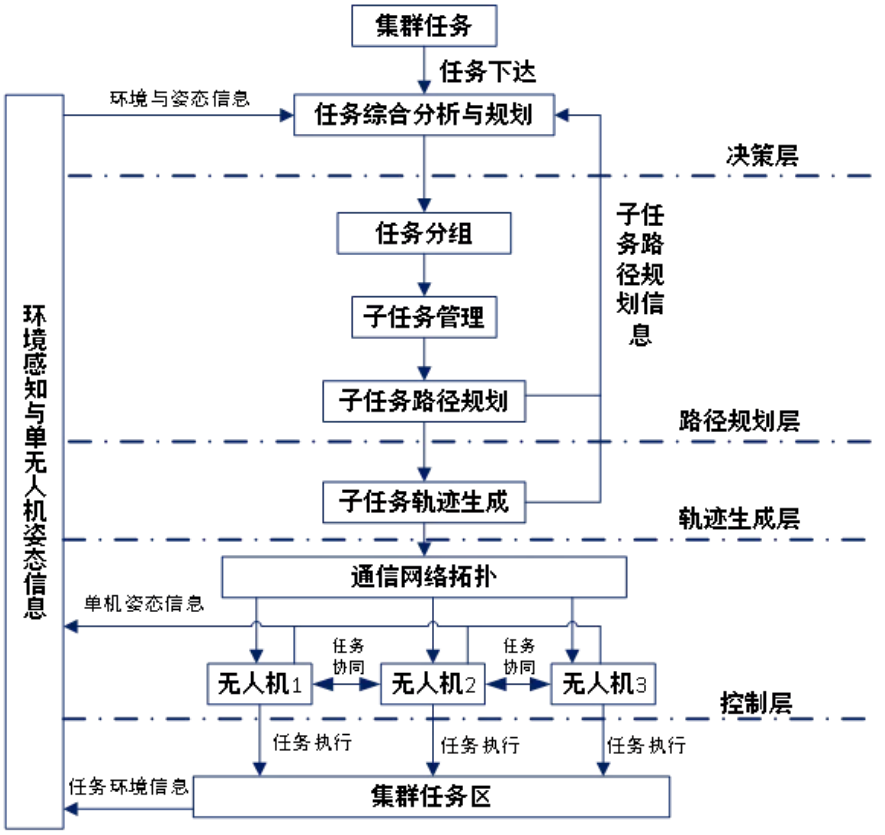
\includegraphics[width=0.9\textwidth]{pictures/formationStruct_1.png}
    \caption{无人机集群任务规划分层结构}
    \label{struct_1}
\end{figure}